%%%%%%%%%%%%%%%%%%%%%%%%%%%%%%%%%%%%%%%%%
% Programming/Coding Assignment
% LaTeX Template
%
% This template has been downloaded from:
% http://www.latextemplates.com
%
% Original author:
% Ted Pavlic (http://www.tedpavlic.com)
%
% Adapted by:
% Jacopo De Stefani (jacopo.de.stefani@gmail.com)
%
% Note:
% The \lipsum[#] commands throughout this template generate dummy text
% to fill the template out. These commands should all be removed when 
% writing assignment content.
%
% This template uses a Perl script as an example snippet of code, most other
% languages are also usable. Configure them in the "CODE INCLUSION 
% CONFIGURATION" section.
%
%%%%%%%%%%%%%%%%%%%%%%%%%%%%%%%%%%%%%%%%%

%----------------------------------------------------------------------------------------
%	PACKAGES AND OTHER DOCUMENT CONFIGURATIONS
%----------------------------------------------------------------------------------------

\documentclass{article}

\usepackage[utf8]{inputenc}
\usepackage{textcomp}
\usepackage{fancyhdr} % Required for custom headers
\usepackage{lastpage} % Required to determine the last page for the footer
\usepackage{extramarks} % Required for headers and footers
\usepackage[usenames,dvipsnames]{color} % Required for custom colors
\usepackage{graphicx} % Required to insert images
\usepackage{listings} % Required for insertion of code
\usepackage{courier} % Required for the courier font
\usepackage{lipsum} % Used for inserting dummy 'Lorem ipsum' text into the template
\usepackage{rotating}
\usepackage{natbib}
\usepackage{graphicx}
\usepackage{tikz}
\usepackage{pgfplots}
\usepackage{multicol}
\usepackage{caption}
\usepackage{amsmath}
\usepackage{amsfonts}
\usepackage{algpseudocode}% http://ctan.org/pkg/algorithmicx
\usepackage{algorithm}% http://ctan.org/pkg/algorithm
\usepackage{pdflscape}
\usepackage{hyperref}
\usepackage{pifont}
\usepackage{subcaption}

\usetikzlibrary{positioning,shadows,arrows,intersections,calc,automata}

% Margins
\topmargin=-0.45in
\evensidemargin=0in
\oddsidemargin=0in
\textwidth=6.5in
\textheight=9.0in
\headsep=0.25in

\linespread{1.1} % Line spacing

% Set up the header and footer
\pagestyle{fancy}
\lhead{} % Top left header
\chead{\hmwkClass\ (\hmwkClassInstructor\ ): \hmwkTitle} % Top center head
\rhead{}%\firstxmark} % Top right header
\lfoot{\hmwkAuthorName} % Bottom left footer
\cfoot{}%\lastxmark} % Bottom center footer
\rfoot{Page\ \thepage\ of\ \protect\pageref{LastPage}} % Bottom right footer
\renewcommand\headrulewidth{0.4pt} % Size of the header rule
\renewcommand\footrulewidth{0.4pt} % Size of the footer rule

\setlength\parindent{0pt} % Removes all indentation from paragraphs

%----------------------------------------------------------------------------------------
%	CODE INCLUSION CONFIGURATION
%----------------------------------------------------------------------------------------

\definecolor{MyDarkGreen}{rgb}{0.0,0.4,0.0} % This is the color used for comments
\lstloadlanguages{Python} % Load Perl syntax for listings, for a list of other languages supported see: ftp://ftp.tex.ac.uk/tex-archive/macros/latex/contrib/listings/listings.pdf
\lstset{language=Python, % Use Perl in this example
        frame=single, % Single frame around code
        basicstyle=\small\ttfamily, % Use small true type font
        keywordstyle=[1]\color{Blue}\bf, % Perl functions bold and blue
        keywordstyle=[2]\color{Purple}, % Perl function arguments purple
        keywordstyle=[3]\color{Blue}\underbar, % Custom functions underlined and blue
        identifierstyle=, % Nothing special about identifiers                                         
        commentstyle=\usefont{T1}{pcr}{m}{sl}\color{MyDarkGreen}\small, % Comments small dark green courier font
        stringstyle=\color{Purple}, % Strings are purple
        showstringspaces=false, % Don't put marks in string spaces
        tabsize=5, % 5 spaces per tab
        %
        % Put standard Perl functions not included in the default language here
        morekeywords={rand},
        %
        % Put Perl function parameters here
        morekeywords=[2]{on, off, interp},
        %
        % Put user defined functions here
        morekeywords=[3]{test},
       	%
        morecomment=[l][\color{Blue}]{...}, % Line continuation (...) like blue comment
        numbers=left, % Line numbers on left
        firstnumber=1, % Line numbers start with line 1
        numberstyle=\tiny\color{Blue}, % Line numbers are blue and small
        stepnumber=5, % Line numbers go in steps of 5
        breaklines=true
}

% Creates a new command to include a perl script, the first parameter is the filename of the script (without .pl), the second parameter is the caption
\newcommand{\pyscript}[2]{
\begin{itemize}
\item[]\lstinputlisting[caption=#2,label=#1]{#1.py}
\end{itemize}
}

%----------------------------------------------------------------------------------------
%	DOCUMENT STRUCTURE COMMANDS
%	Skip this unless you know what you're doing
%----------------------------------------------------------------------------------------

% Header and footer for when a page split occurs within a problem environment
\newcommand{\enterProblemHeader}[1]{
\nobreak\extramarks{#1}{#1 continued on next page\ldots}\nobreak
\nobreak\extramarks{#1 (continued)}{#1 continued on next page\ldots}\nobreak
}

% Header and footer for when a page split occurs between problem environments
\newcommand{\exitProblemHeader}[1]{
\nobreak\extramarks{#1 (continued)}{#1 continued on next page\ldots}\nobreak
\nobreak\extramarks{#1}{}\nobreak
}

\setcounter{secnumdepth}{0} % Removes default section numbers
\newcounter{homeworkProblemCounter} % Creates a counter to keep track of the number of problems

\newcommand{\homeworkProblemName}{}
\newenvironment{homeworkProblem}[1][Problem \arabic{homeworkProblemCounter}]{ % Makes a new environment called homeworkProblem which takes 1 argument (custom name) but the default is "Problem #"
\stepcounter{homeworkProblemCounter} % Increase counter for number of problems
\renewcommand{\homeworkProblemName}{#1} % Assign \homeworkProblemName the name of the problem
\section{\homeworkProblemName} % Make a section in the document with the custom problem count
\enterProblemHeader{\homeworkProblemName} % Header and footer within the environment
}{
\exitProblemHeader{\homeworkProblemName} % Header and footer after the environment
}

\newcommand{\problemAnswer}[1]{ % Defines the problem answer command with the content as the only argument
\noindent\framebox[\columnwidth][c]{\begin{minipage}{0.98\columnwidth}#1\end{minipage}} % Makes the box around the problem answer and puts the content inside
}

\newcommand{\homeworkSectionName}{}
\newenvironment{homeworkSection}[1]{ % New environment for sections within homework problems, takes 1 argument - the name of the section
\renewcommand{\homeworkSectionName}{#1} % Assign \homeworkSectionName to the name of the section from the environment argument
\subsection{\homeworkSectionName} % Make a subsection with the custom name of the subsection
\enterProblemHeader{\homeworkProblemName\ [\homeworkSectionName]} % Header and footer within the environment
}{
\enterProblemHeader{\homeworkProblemName} % Header and footer after the environment
}

%----------------------------------------------------------------------------------------
%	USER DEFINED TIKZ STYLES
%----------------------------------------------------------------------------------------

\tikzset{
    player1/.style={circle, draw=none, fill=green!70!black, circular drop shadow,
        text centered, anchor=north, text=white},
    player2/.style={circle, draw=none, fill=orange, circular drop shadow,
        text centered, anchor=north, text=white},
    chance/.style={circle, draw,text centered, anchor=north},
    subtreeB/.style={rectangle, draw, rounded corners=1mm, color=red, thick,
        text centered, anchor=north, text=red},
    subtreeC/.style={rectangle, draw, rounded corners=1mm, color=orange, thick,
        text centered, anchor=north, text=orange},
    ex2/.style={circle, draw,text centered, anchor=north},
    nashEq1P/.style={circle,draw=none, fill=green!70!black, text centered, anchor=north, text=white,inner sep=2pt},
    nashEq2P/.style={circle,draw=none, fill=orange, text centered, anchor=north, text=white,inner sep=2pt},
    nashEqPoints/.style={fill=white,draw=black,thick},
    level distance=0.5cm, growth parent anchor=south
}

\tikzstyle{tier}=[draw, fill=yellow!20, text width=6.0em, text centered,
  minimum height=1.5em,drop shadow]
\tikzstyle{component} = [tier, text width=8em, minimum width=10em,
  minimum height=3em, rounded corners, drop shadow,inner sep=2pt]
\tikzstyle{texto} = [above, text width=6em, text centered]
\tikzstyle{linepart} = [draw, thick, color=black!50, -latex', dashed]
\tikzstyle{line} = [draw, thick, color=black!50, -latex', ->]
\tikzstyle{ur}=[draw, text centered, minimum height=0.01em]
 
% Define distances for bordering
\newcommand{\blockdist}{1.3}
\newcommand{\edgedist}{1.5}

\newcommand{\component}[2]{node (p#1) [component]
  {{\scriptsize\textit{#2}}}}


% Draw background
\newcommand{\backgroundSquare}[5]{%
  \begin{pgfonlayer}{background}
    % Left-top corner of the background rectangle
    \path (#1.west |- #2.north)+(-0.5,0.5) node (a1) {};
    % Right-bottom corner of the background rectanle
    \path (#3.east |- #4.south)+(+0.5,-0.25) node (a2) {};
    % Draw the background
    \path[fill=blue!20,rounded corners, draw=black!50, dashed]
      (a1) rectangle (a2);
    \path (a1.east |- a1.south)+(0.8,-0.3) node (u1)[texto]
      {\scriptsize\textit{#5 Tier}};
  \end{pgfonlayer}}


\newcommand*\circled[2]{\tikz[baseline=(char.base)]{
            \node[#2,rectangle, rounded corners=0.7mm, text=white] (char) {#1};}}
\newcommand*\cellvcenter[1]{\raisebox{-\height}{#1}}


\newcommand{\cmark}{\ding{51}}%
\newcommand{\xmark}{\ding{55}}%

%----------------------------------------------------------------------------------------
%	NAME AND CLASS SECTION
%----------------------------------------------------------------------------------------

\newcommand{\hmwkTitle}{Implementation Exercise \#2 \\ The Traveling Salesman Problem with Time Windows - Stochastic Local Search Algorithms} % Assignment title
\newcommand{\hmwkDueDate}{Wednesday,\ April\ 10,\ 2013} % Due date
\newcommand{\hmwkClass}{INFO-H-413 - Learning Dynamics} % Course/class
\newcommand{\hmwkClassTime}{} % Class/lecture time
\newcommand{\hmwkClassInstructor}{Prof. T. St\"{u}etzle} % Teacher/lecturer
\newcommand{\hmwkAuthorName}{Jacopo De Stefani} % Your name
\newcommand{\maxmin}{$\mathcal{MAX}-\mathcal{MIN}$}

%----------------------------------------------------------------------------------------
%	TITLE PAGE
%----------------------------------------------------------------------------------------

\title{
\vspace{2in}
\textmd{\textbf{\hmwkClass:\\ \hmwkTitle}}\\
%\normalsize\vspace{0.1in}\small{Due\ on\ \hmwkDueDate}\\
\vspace{0.1in}\large{\textit{\hmwkClassInstructor\ }}
\vspace{3in}
}

\author{\textbf{\hmwkAuthorName}}
\date{\today} % Insert date here if you want it to appear below your name

%----------------------------------------------------------------------------------------

\begin{document}

\maketitle

%----------------------------------------------------------------------------------------
%	TABLE OF CONTENTS
%----------------------------------------------------------------------------------------

%\setcounter{tocdepth}{1} % Uncomment this line if you don't want subsections listed in the ToC

\newpage
\tableofcontents
\newpage

\section{Implementation}
The heuristic solver had been written using the C++ programming language, in order to be able to take adventage of the functionalities offered by the Standard Template Library (STL).

By combining an object-oriented approach with those functionalities, I built a modular application core (\emph{HeuristicCore}) that has been used for the two exercises required for this implementation.

The core is directly linked with the reader (\emph{InstanceReader}) which reads the files containing all the informations to run the simulation (distance matrix, time windows vector and seeds list) and the writer (\emph{Writer}) which outputs the results of the simulation in a CSV file.

Two different command line front-ends, sharing the same underlying structure, but having a different set of parameters, have been developed to distinguish the iterative-improvement interface from the variable neighborhood descent one. 

The global program structure is depicted here:

\begin{center}
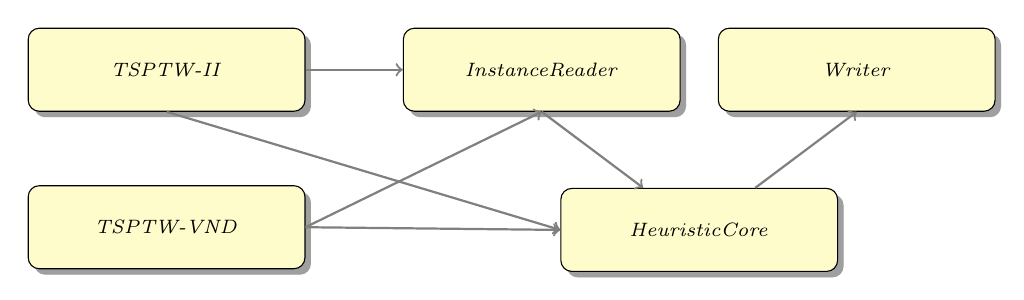
\begin{tikzpicture}[transform shape]
 
  % Draw diagram elements
  
  \path \component {1}{HeuristicCore};
  \path (p1.north)+(-2.0,+1.5) \component{2}{InstanceReader};
  \path (p1.north)+(+2.0,+1.5) \component{3}{Writer};
  \path (p2.west)+(-3.0,0.0) \component{4}{TSPTW-II};
  \path (p2.west)+(-3.0,-2.0) \component{5}{TSPTW-VND}; 
     
  % Draw arrows between elements
  \path [line] (p2.south) -> node [above] {} (p1);
  \path [line] (p1) -> node [above, midway] {} (p3.south);
  \path [line] (p4.east) -> node [above] {} (p2.west);
  \path [line] (p5.east) -> node [above] {} (p2.south);
  \path [line] (p4.south) -> node [above] {} (p1.west);
  \path [line] (p5.east) -> node [above] {} (p1.west);
  
  %\backgroundSquare{p1}{p1}{p3}{p3}{Presentation}

 \end{tikzpicture}
 \captionof{figure}{Simulation Code Structure}
\end{center}

The names of the nodes corresponds to those of the implementation (.cpp) and header files for the corresponding classes.
In addition to these, a class to represent the time windows (TimeWindow.h) and another one to represent the candidate solution as
a user defined data type (CandidateSolution.\{h,cpp\}) have been implemented.


\subsection{How to compile the program?}
The software was developed in C++98 under Linux (Debian Wheezy), using the GNU g++ (Debian 4.7.2-5) 4.7.2 compiler and tested in this environment. 
The software is distributed as a compressed tar file, containing both the source code (in the \verb|src| folder) and the scripts and instances (in the \verb|bin| and \verb|bin\instances| respectively).
To install the program, first obtain the file TSPTW.V1.0.tar.gz. 

Unzip the file by typing:

\begin{center}
\begin{verbatim}
gunzip TSPTW.V1.0.tar.gz
\end{verbatim}
\end{center}

and then unpack it by typing:

\begin{center}
\begin{verbatim}
tar -xvf TSPTW.V1.0.tar
\end{verbatim}
\end{center}

The software will be extracted in a new folder TSPTW.V1.0 

Finally, by launching
\begin{center}
\begin{verbatim}
make all
\end{verbatim}
\end{center}

the Makefile will trigger the compilation of the files,
producing the executables 'TSPTW-II' and 'TSPTW-VND" in the \verb|bin| folder.

\textbf{Note:} The code is written in C++98. Hence, the code should be
reasonable portable to other Operating Systems than Linux or Unix.

\subsection{How to run the program?}

Once the program has been compiled, two separate executable files,
corresponding to the different kind of metaheuristic (i.e. Iterative Improvement
and Variable Neighborhood Descent) can be either launched directly via the command line
interface or using the bash script to launch.

The design choice to separate the two different kind of metaheuristic is made in order to limit the number of command line parameters to be given as input to the program.

\subsubsection{Command-line execution}
By launching\footnote{The squared-bracket notation implies that the formal parameters to the script have to be substituted by their actual value.}:
\begin{center}
\begin{verbatim}
./TSPTW-II [PARAMETERS] -i [INPUT_FILE] -s [SEEDS_FILE]
\end{verbatim}
\begin{verbatim}
./TSPTW-VND [PARAMETERS] -i [INPUT_FILE] -s [SEEDS_FILE]
\end{verbatim}
\end{center}

one can display the information about the meaning of the different options that can be given as input to the program.

Additional information concerning the usage of the program can be found in the README file.

The only mandatory options are "-i, --input" and "-s,-seeds", since
without these components will not be possible to execute the simulation.

The argument to the input option must contain the full path to the instance file.

The seeds file must contain a number of seeds at least equal to the number of
runs required, one seed per line without any additional information.

The options controlling the same parameters are mutually exclusive, with that
meaning that only one option must be selected in order to run the program.
If multiple options for the same parameter are chosen, the program will not
run.

\paragraph{TSPTW-II}
\begin{tabular}{|l|c|}
\hline
\textbf{Parameter}	&	\textbf{Mutually exclusive options} \\ \hline
Initial solution & -d,--random , -h,--heuristic \\ \hline
Neighborhood type &-t,--transpose , -e,--exchange , -n,--insert \\ \hline 
Pivoting rule &	-f,--first-imp , -b,--best-imp \\ \hline
\end{tabular}

\paragraph{TSPTW-VND}

\begin{tabular}{|l|c|}
\hline
\textbf{Parameter}	&	\textbf{Mutually exclusive options} \\ \hline
VND algorithm & -t,--standard , -p,--piped \\ \hline
Neighborhood chain & 	-a,--TEI  , -b,--TIE \\ \hline
\end{tabular}

\paragraph{Output}
Every experiment produces a single file:
\begin{itemize}
  \item \textbf{(II)} $[pivoting\_rule].[neighborhood\_type].[INSTANCE\_NAME]$ with $[pivoting\_rule] \in \{first,best\}$ and $[neighborhood\_type] \in \{transpose,exchange,insert\}$ 
  \item \textbf{(VND)} $[vnd\_type].[neighborhood\_chain].[INSTANCE\_NAME]$ with $[vnd\_type] \in \{standard,piped\}$ and $[neighborhood\_type] \in \{tei,tie\}$
\end{itemize} 
				
					 
\textbf{Examples:} \begin{verbatim}
exchange.best.n80w200.004.txt
standard.tei.n80w20.003.txt
\end{verbatim}


The internal structure of the file is the following: \begin{tabular}{|c|c|c|c|}
\hline
\textbf{Seed}	&	\textbf{CV} & \textbf{CpuTime} & \textbf{PRPD} \\ \hline
\end{tabular}

For each run of the algorithm, the program writes in the file, using a tabulation as separator,
the used seed, the number of constraints violations, the cpu runtime and the penalised relative percentage deviation.


\subsubsection{Script execution}
By launching:
\begin{center}
\begin{verbatim}
./launchTSPTW-II.sh [INSTANCE_NAME] [RUNS] [SEEDS_FILE]
\end{verbatim}
\begin{verbatim}
./launchTSPTW-VND.sh [INSTANCE_NAME] [RUNS] [SEEDS_FILE]
\end{verbatim}
\end{center}

The script will:
\begin{enumerate}
  \item Create the files required by the data processing script to write statistics.
  \item Generate a seed file, named [SEEDS\_FILE] containing [RUNS] randomly generated seeds.
  \item Launch the corresponding TSPTW program for [RUNS]  using all the possible combinations of input options.
  \item Wait for the termination of all the previously launched experiment and call the R data processing script
\end{enumerate}

The script assumes that all the instances are located into the instances folder, hence it is only necessary to indicate the instance name, instead of the complete path.

\paragraph{Output}

Each execution of the script will then generate the files:
\begin{itemize}
  \item $[INSTANCE\_NAME]-CpuTime.pdf$ containing the boxplots of the runtime distribution for each algorithm.
  \item $[INSTANCE\_NAME]-PRPD.pdf$ containing the boxplots of the PRPD distribution for each algorithm.
  \item 
        \begin{itemize}
          \item \textbf{(II)} transpose.first, exchange.first, insert.first, transpose.best, exchange.best, insert.best 
          \item \textbf{(VND)} standard.tei, standard.tie, piped.tei, piped.tie
        \end{itemize}
\end{itemize}

The internal structure of the file is the following:

 
\begin{tabular}{|c|c|c|c|}
\hline
\textbf{Instance}	&	\textbf{Infeasible} & \textbf{mean(PRDP)} &	\textbf{mean(CpuTime)} \\ \hline
\end{tabular}

Each line contains the instance name, the percentage of infeasible runs, the mean PRDP and the mean runtime across [RUNS] runs.

%%----------------------------------------------------------------------------------------
%	PROBLEM 1
%----------------------------------------------------------------------------------------

% To have just one problem per page, simply put a \clearpage after each problem
\newpage
\begin{homeworkProblem}
\section{Iterative improvement algorithms}
\subsection{Problem statement}
Implement iterative improvement algorithms with:
\begin{itemize}
  \item first-improvement
  \item best-improvement
\end{itemize}
pivoting rule for each of the three neighborhoods: transpose, exchange, and insert. \\
As a starting solution for iterative improvement, consider a random permutation, that is, use the method “Uninformed Random Picking” (see slides of lectures). Bonus points will be awarded for also considering an insertion heuristic as an alternative to random initialization.
\begin{enumerate}
  \item Run the 6 resulting iterative improvement algorithms (all combinations of the two pivoting rules and the
three neighborhoods) on each of the instances. Repeat each run 100 times with different seed for the random
number generator.
\item Compute the following statistics for each of the 6 iterative improvement algorithms and each instance:
\begin{itemize}
  \item Percentage of runs with constraint violations
  \item Mean penalised relative percentage deviation
  \item Mean computation time
\end{itemize} 
\item Produce boxplots of penalised relative percentage deviation and computation time per instance.
\item Determine using statistical tests (in this case, the Wilcoxon test), whether there is a statistically significant difference between the quality of the solutions generated by the different algorithms.
In particular, compare best vs. first-improvement for each neighborhood, and exchange vs. insertion for each pivoting rule.
\end{enumerate}

\subsection{Experiment results}
\subsubsection{n80w20.001}
\begin{center}
\includegraphics[width=0.6\textwidth,keepaspectratio]{{II/n80w20.001/n80w20.001-CpuTime}.pdf}
\captionof{figure}{n80w20.001 - Runtime boxplots for the different iterative improvement algorithms}
\end{center}

\begin{center}
\includegraphics[width=0.6\textwidth,keepaspectratio]{{II/n80w20.001/n80w20.001-PRPD}.pdf}
\captionof{figure}{n80w20.001 - PRPD boxplots for the different iterative improvement algorithms}
\end{center}

\begin{center}
\begin{tabular}{|l|l|}
\hline
\textbf{Test} & \textbf{P-Value} \\
\hline
First vs best - Transpose&9.74631639820544e-18\\
\hline
First vs best - Exchange&2.04966732989559e-17\\
\hline
First vs best - Insert&1.74838327736385e-15\\
\hline
Exchange vs Insert - First&3.95591160889952e-18\\
\hline
Exchange vs Insert - Best&3.9556885406462e-18\\
\hline
\end{tabular}
\captionof{table}{n80w20.001 - Results of Wilcoxon paired signed rank test}
\end{center}

\subsubsection{n80w20.002}
\begin{center}
\includegraphics[width=0.6\textwidth,keepaspectratio]{{II/n80w20.002/n80w20.002-CpuTime}.pdf}
\captionof{figure}{n80w20.002 - Runtime boxplots for the different iterative improvement algorithms}
\end{center}

\begin{center}
\includegraphics[width=0.6\textwidth,keepaspectratio]{{II/n80w20.002/n80w20.002-PRPD}.pdf}
\captionof{figure}{n80w20.002 - PRPD boxplots for the different iterative improvement algorithms}
\end{center}

\begin{center}
\begin{tabular}{|l|l|}
\hline
\textbf{Test} & \textbf{P-Value} \\
\hline
First vs best - Transpose&3.95591160889952e-18\\
\hline
First vs best - Exchange&1.61703099974578e-17\\
\hline
First vs best - Insert&2.39050570998277e-07\\
\hline
Exchange vs Insert - First&3.95591160889952e-18\\
\hline
Exchange vs Insert - Best&3.9556885406462e-18\\
\hline
\end{tabular}
\captionof{table}{n80w20.002 - Results of Wilcoxon paired signed rank test}
\end{center}

\subsubsection{n80w20.003}
\begin{center}
\includegraphics[width=0.6\textwidth,keepaspectratio]{{II/n80w20.003/n80w20.003-CpuTime}.pdf}
\captionof{figure}{n80w20.003 - Runtime boxplots for the different iterative improvement algorithms}
\end{center}

\begin{center}
\includegraphics[width=0.6\textwidth,keepaspectratio]{{II/n80w20.003/n80w20.003-PRPD}.pdf}
\captionof{figure}{n80w20.003 - PRPD boxplots for the different iterative improvement algorithms}
\end{center}

\begin{center}
\begin{tabular}{|l|l|}
\hline
\textbf{Test} & \textbf{P-Value} \\
\hline
First vs best - Transpose&3.95591160889952e-18\\
\hline
First vs best - Exchange&6.21747363653032e-18\\
\hline
First vs best - Insert&6.2952945764779e-08\\
\hline
Exchange vs Insert - First&3.9556885406462e-18\\
\hline
Exchange vs Insert - Best&3.95591160889952e-18\\
\hline
\end{tabular}
\captionof{table}{n80w20.003 - Results of Wilcoxon paired signed rank test}
\end{center}

\subsubsection{n80w20.004}
\begin{center}
\includegraphics[width=0.6\textwidth,keepaspectratio]{{II/n80w20.004/n80w20.004-CpuTime}.pdf}
\captionof{figure}{n80w20.004 - Runtime boxplots for the different iterative improvement algorithms}
\end{center}

\begin{center}
\includegraphics[width=0.6\textwidth,keepaspectratio]{{II/n80w20.004/n80w20.004-PRPD}.pdf}
\captionof{figure}{n80w20.001 - PRPD boxplots for the different iterative improvement algorithms}
\end{center}

\begin{center}
\begin{tabular}{|l|l|}
\hline
\textbf{Test} & \textbf{P-Value} \\
\hline
First vs best - Transpose&4.33123080260219e-18\\
\hline
First vs best - Exchange&1.5356610755813e-16\\
\hline
First vs best - Insert&4.27702026764362e-14\\
\hline
Exchange vs Insert - First&5.59593516960623e-18\\
\hline
Exchange vs Insert - Best&3.95591160889952e-18\\
\hline
\end{tabular}
\captionof{table}{n80w20.004 - Results of Wilcoxon paired signed rank test}
\end{center}

\subsubsection{n80w20.005}
\begin{center}
\includegraphics[width=0.6\textwidth,keepaspectratio]{{II/n80w20.005/n80w20.005-CpuTime}.pdf}
\captionof{figure}{n80w20.005 - Runtime boxplots for the different iterative improvement algorithms}
\end{center}

\begin{center}
\includegraphics[width=0.6\textwidth,keepaspectratio]{{II/n80w20.005/n80w20.005-PRPD}.pdf}
\captionof{figure}{n80w20.005 - PRPD boxplots for the different iterative improvement algorithms}
\end{center}

\begin{center}
\begin{tabular}{|l|l|}
\hline
\textbf{Test} & \textbf{P-Value} \\
\hline
First vs best - Transpose&4.46398542390809e-18\\
\hline
First vs best - Exchange&4.74166029806301e-18\\
\hline
First vs best - Insert&4.0369131744045e-10\\
\hline
Exchange vs Insert - First&4.74166029806301e-18\\
\hline
Exchange vs Insert - Best&3.95591160889952e-18\\
\hline
\end{tabular}
\captionof{table}{n80w20.005 - Results of Wilcoxon paired signed rank test}
\end{center}

\subsubsection{n80w200.001}
\begin{center}
\includegraphics[width=0.6\textwidth,keepaspectratio]{{II/n80w200.001/n80w200.001-CpuTime}.pdf}
\captionof{figure}{n80w200.001 - Runtime boxplots for the different iterative improvement algorithms}
\end{center}

\begin{center}
\includegraphics[width=0.6\textwidth,keepaspectratio]{{II/n80w200.001/n80w200.001-PRPD}.pdf}
\captionof{figure}{n80w200.001 - PRPD boxplots for the different iterative improvement algorithms}
\end{center}

\begin{center}
\begin{tabular}{|l|l|}
\hline
\textbf{Test} & \textbf{P-Value} \\
\hline
First vs best - Transpose&4.07730530936212e-18\\
\hline
First vs best - Exchange&2.17457280454137e-17\\
\hline
First vs best - Insert&3.95591160889952e-18\\
\hline
Exchange vs Insert - First&3.95591160889952e-18\\
\hline
Exchange vs Insert - Best&3.95591160889952e-18\\
\hline
\end{tabular}
\captionof{table}{n80w200.001 - Results of Wilcoxon paired signed rank test}
\end{center}

\subsubsection{n80w200.002}
\begin{center}
\includegraphics[width=0.6\textwidth,keepaspectratio]{{II/n80w200.002/n80w200.002-CpuTime}.pdf}
\captionof{figure}{n80w200.002 - Runtime boxplots for the different iterative improvement algorithms}
\end{center}

\begin{center}
\includegraphics[width=0.6\textwidth,keepaspectratio]{{II/n80w200.002/n80w200.002-PRPD}.pdf}
\captionof{figure}{n80w200.002 - PRPD boxplots for the different iterative improvement algorithms}
\end{center}

\begin{center}
\begin{tabular}{|l|l|}
\hline
\textbf{Test} & \textbf{P-Value} \\
\hline
First vs best - Transpose&5.19043683699158e-18\\
\hline
First vs best - Exchange&4.6720416035814e-17\\
\hline
First vs best - Insert&3.95591160889952e-18\\
\hline
Exchange vs Insert - First&3.95591160889952e-18\\
\hline
Exchange vs Insert - Best&3.95591160889952e-18\\
\hline
\end{tabular}
\captionof{table}{n80w200.002 - Results of Wilcoxon paired signed rank test}
\end{center}

\subsubsection{n80w200.003}
\begin{center}
\includegraphics[width=0.6\textwidth,keepaspectratio]{{II/n80w200.003/n80w200.003-CpuTime}.pdf}
\captionof{figure}{n80w200.003 - Runtime boxplots for the different iterative improvement algorithms}
\end{center}

\begin{center}
\includegraphics[width=0.6\textwidth,keepaspectratio]{{II/n80w200.003/n80w200.003-PRPD}.pdf}
\captionof{figure}{n80w200.003 - PRPD boxplots for the different iterative improvement algorithms}
\end{center}

\begin{center}
\begin{tabular}{|l|l|}
\hline
\textbf{Test} & \textbf{P-Value} \\
\hline
First vs best - Transpose&4.33123080260219e-18\\
\hline
First vs best - Exchange&7.01070639830382e-18\\
\hline
First vs best - Insert&3.95591160889952e-18\\
\hline
Exchange vs Insert - First&3.95591160889952e-18\\
\hline
Exchange vs Insert - Best&3.95591160889952e-18\\
\hline
\end{tabular}
\captionof{table}{n80w200.003 - Results of Wilcoxon paired signed rank test}
\end{center}

\subsubsection{n80w200.004}
\begin{center}
\includegraphics[width=0.6\textwidth,keepaspectratio]{{II/n80w200.004/n80w200.004-CpuTime}.pdf}
\captionof{figure}{n80w200.004 - Runtime boxplots for the different iterative improvement algorithms}
\end{center}

\begin{center}
\includegraphics[width=0.6\textwidth,keepaspectratio]{{II/n80w200.004/n80w200.004-PRPD}.pdf}
\captionof{figure}{n80w200.001 - PRPD boxplots for the different iterative improvement algorithms}
\end{center}

\begin{center}
\begin{tabular}{|l|l|}
\hline
\textbf{Test} & \textbf{P-Value} \\
\hline
First vs best - Transpose&4.33123080260219e-18\\
\hline
First vs best - Exchange&2.4473398426105e-17\\
\hline
First vs best - Insert&3.95591160889952e-18\\
\hline
Exchange vs Insert - First&3.95591160889952e-18\\
\hline
Exchange vs Insert - Best&3.95591160889952e-18\\
\hline
\end{tabular}
\captionof{table}{n80w200.004 - Results of Wilcoxon paired signed rank test}
\end{center}

\subsubsection{n80w200.005}
\begin{center}
\includegraphics[width=0.6\textwidth,keepaspectratio]{{II/n80w200.005/n80w200.005-CpuTime}.pdf}
\captionof{figure}{n80w200.005 - Runtime boxplots for the different iterative improvement algorithms}
\end{center}

\begin{center}
\includegraphics[width=0.6\textwidth,keepaspectratio]{{II/n80w200.005/n80w200.005-PRPD}.pdf}
\captionof{figure}{n80w200.005 - PRPD boxplots for the different iterative improvement algorithms}
\end{center}

\begin{center}
\begin{tabular}{|l|l|}
\hline
\textbf{Test} & \textbf{P-Value} \\
\hline
First vs best - Transpose&4.74166029806301e-18\\
\hline
First vs best - Exchange&1.40854365025687e-16\\
\hline
First vs best - Insert&3.95591160889952e-18\\
\hline
Exchange vs Insert - First&3.95591160889952e-18\\
\hline
Exchange vs Insert - Best&3.95591160889952e-18\\
\hline
\end{tabular}
\captionof{table}{n80w200.005 - Results of Wilcoxon paired signed rank test}
\end{center}

\subsection{Statistics}

\subsubsection{Transpose-First Improvement}
\begin{center}
\begin{tabular}{|l|c|l|l|}
\hline
\textbf{Instance}& \textbf{\% Infeasible} & $\mathbf{\bar{PRDP}}$ &$\mathbf{\bar{Runtime}}$\\
\hline
n80w20.001&1&1229712.6&0.0100035563\\
\hline
n80w20.002&1&1028075.17&0.0095843375\\
\hline
n80w20.003&1&1132968.5&0.0098099452\\
\hline
n80w20.005&1&1010681.79&0.0097989762\\
\hline
n80w20.004&1&1226174.6&0.0094877067\\
\hline
n80w200.001&1&1467634.1&0.0098152878\\
\hline
n80w200.002&1&1504523.7&0.0099101404\\
\hline
n80w200.004&1&1388037.6&0.0098893615\\
\hline
n80w200.003&1&1567210.5&0.0097697727\\
\hline
n80w200.005&1&1644110.9&0.0097550971\\
\hline
\end{tabular}
\captionof{table}{Statistics summary for iterative improvement algorithm with Transpose neighborhood and First Improvement pivoting rule}
\end{center}

\subsubsection{Transpose-Best Improvement}
\begin{center}
\begin{tabular}{|l|c|l|l|}
\hline
\textbf{Instance}& \textbf{\% Infeasible} & $\mathbf{\bar{PRDP}}$ &$\mathbf{\bar{Runtime}}$\\
\hline
n80w20.001&1&1236039.3&0.014545497\\
\hline
n80w20.002&1&1033090.48&0.0145450422\\
\hline
n80w20.003&1&1137758.7&0.014536776\\
\hline
n80w20.005&1&1014818.46&0.014947609\\
\hline
n80w20.004&1&1232996&0.015151286\\
\hline
n80w200.001&1&1476994.8&0.0147534638\\
\hline
n80w200.002&1&1511281&0.014884921\\
\hline
n80w200.004&1&1392023.3&0.0146445173\\
\hline
n80w200.003&1&1575355.5&0.0143582468\\
\hline
n80w200.005&1&1653419.6&0.0150098656\\
\hline
\end{tabular}
\captionof{table}{Statistics summary for iterative improvement algorithm with Transpose neighborhood and Best Improvement pivoting rule}
\end{center}

\subsubsection{Exchange-First Improvement}
\begin{center}
\begin{tabular}{|l|c|l|l|}
\hline
\textbf{Instance}& \textbf{\% Infeasible} & $\mathbf{\bar{PRDP}}$ &$\mathbf{\bar{Runtime}}$\\
\hline
n80w20.001&1&1035718.78&18.390814\\
\hline
n80w20.002&1&884386.3&18.198632\\
\hline
n80w20.003&1&956518.77&18.913801\\
\hline
n80w20.005&1&849054.52&19.043496\\
\hline
n80w20.004&1&1030411.56&19.660314\\
\hline
n80w200.001&1&661322.18&23.117446\\
\hline
n80w200.002&1&813339.6&22.552976\\
\hline
n80w200.004&1&679489.06&22.068859\\
\hline
n80w200.003&1&697450.03&24.338257\\
\hline
n80w200.005&1&760027.65&22.348975\\
\hline
\end{tabular}
\captionof{table}{Statistics summary for iterative improvement algorithm with Exchange neighborhood and First Improvement pivoting rule}
\end{center}

\subsubsection{Exchange-Best Improvement}
\begin{center}
\begin{tabular}{|l|c|l|l|}
\hline
\textbf{Instance}& \textbf{\% Infeasible} & $\mathbf{\bar{PRDP}}$ &$\mathbf{\bar{Runtime}}$\\
\hline
n80w20.001&1&1086217.68&13.091453\\
\hline
n80w20.002&1&901762.05&13.365301\\
\hline
n80w20.003&1&1017243.86&13.267128\\
\hline
n80w20.005&1&895720.53&13.5824245\\
\hline
n80w20.004&1&1084080.4&14.189582\\
\hline
n80w200.001&1&1022433.76&16.418229\\
\hline
n80w200.002&1&1075649.94&16.028712\\
\hline
n80w200.004&1&994703.67&15.518766\\
\hline
n80w200.003&1&1094460.9&16.16696\\
\hline
n80w200.005&1&1110949.86&16.566802\\
\hline
\end{tabular}
\captionof{table}{Statistics summary for iterative improvement algorithm with Exchange neighborhood and Best Improvement pivoting rule}
\end{center}

\subsubsection{Insert-First Improvement}
\begin{center}
\begin{tabular}{|l|c|l|l|}
\hline
\textbf{Instance}& \textbf{\% Infeasible} & $\mathbf{\bar{PRDP}}$ &$\mathbf{\bar{Runtime}}$\\
\hline
n80w20.001&0.65&16070.27322082&25.88279\\
\hline
n80w20.002&0.83&11803.71462682&28.509938\\
\hline
n80w20.003&0.83&21587.617&28.579453\\
\hline
n80w20.005&0.32&4945.642107&28.672083\\
\hline
n80w20.004&0.49&10894.01867489&28.474429\\
\hline
n80w200.001&0.22&6119.9927045&59.544212\\
\hline
n80w200.002&0&11.2561521&64.580306\\
\hline
n80w200.004&0.11&3049.80805246&63.942238\\
\hline
n80w200.003&0.01&437.87774695&63.687806\\
\hline
n80w200.005&0.01&464.62990671&66.084369\\
\hline

\end{tabular}
\captionof{table}{Statistics summary for iterative improvement algorithm with Insert neighborhood and First Improvement pivoting rule}
\end{center}

\subsubsection{Insert-Best Improvement}
\begin{center}
\begin{tabular}{|l|c|l|l|}
\hline
\textbf{Instance}& \textbf{\% Infeasible} & $\mathbf{\bar{PRDP}}$ &$\mathbf{\bar{Runtime}}$\\
\hline
n80w20.001&0.56&14772.44442862&28.769951\\
\hline
n80w20.002&0.84&16009.51797952&30.159812\\
\hline
n80w20.003&0.89&26984.256&30.197019\\
\hline
n80w20.005&0.52&10159.3062354&30.776906\\
\hline
n80w20.004&0.59&18861.32619536&31.013\\
\hline
n80w200.001&0.37&21195.2243605&33.031965\\
\hline
n80w200.002&0&13.2172159&33.011011\\
\hline
n80w200.004&0.42&23019.4946845&34.123681\\
\hline
n80w200.003&0.12&7740.06242146&34.080592\\
\hline
n80w200.005&0.07&2516.0079072&33.450537\\
\hline
\end{tabular}
\captionof{table}{Statistics summary for iterative improvement algorithm with Insert neighborhood and Best Improvement pivoting rule}
\end{center}

\end{homeworkProblem}		

%----------------------------------------------------------------------------------------
%	PROBLEM 1
%----------------------------------------------------------------------------------------

% To have just one problem per page, simply put a \clearpage after each problem
\newpage
\begin{homeworkProblem}
\section{Ant Colony Optimization} \label{aco}
\subsection{Problem statement}
Implement two stochastic local search (SLS) algorithms for the traveling salesman problem with time windows (TPSTW), building on top of the perturbative local search methods from the first implementation exercise.
\begin{enumerate}
  \item Run each algorithm 25 times with different random seed on each instance. Instances will be available from http://iridia.ulb.ac.be/˜stuetzle/Teaching/HO/. As termination criterion, for each instance, use the maximum computation time it takes to run a full VND (implemented in the previous exercise) on the same instance and then multiply this time by 1000 (to allow for long enough runs of the SLS algorithms).
 \item Compute the following statistics for each of the two SLS algorithms and each instance:
 \begin{itemize}
   \item Percentage of runs with constraint violations
   \item Mean penalized relative percentage deviation
 \end{itemize}

\item Produce box-plots of penalized relative percentage deviation.
\item Determine, using statistical tests (in this case, the Wilcoxon test), whether there is a statistically significant difference between the quality of the solutions generated by the two algorithms.
\item Measure, for each of the implemented algorithms on 5 instances, the run-time distributions to reach sufficiently high quality solutions (e.g. best-known solutions available at http://iridia.ulb.ac.be/˜manuel/tsptw-instances\#instances).
Measure the run-time distributions across 25 repetitions using a cut-off time of 10 times the termination criterion above.
\item Produce a written report on the implementation exercise:
\begin{itemize}
  \item Please make sure that each implemented SLS algorithm is appropriately described and that the computational results are carefully interpreted. Justify also the choice of the parameter settings and the choice
of the iterative improvement algorithm for the hybrid SLS algorithm.
  \item Present the results as in the previous implementation exercise (tables, box-plots, statistical tests).
  \item Present graphically the results of the analysis of the run-time distributions.
  \item Interpret appropriately the results and make conclusions on the relative performance of the algorithms across all the benchmark instances studied.
\end{itemize}
\end{enumerate}

\subsection{Introduction} \label{sec:introACO}
Ant Colony Optimization is an example of population-based metaheuristic (i.e a set of algorithmic concepts that can be used to define heuristic methods) inspired by the behavior of the ant species \emph{Iridomyrmex humilis}.

To be more precise, these insects are able, by means of stigmergic communication, to choose the shortest path between their nest and a food source, when given the choice (\cite{deneubourg1990self}).

The communication process occurs by deposing a certain quantity of pheromone in the environment that can be sensed by the other ants and that will be used by them as an heuristic (i.e an information to guide their choice) for selecting the shortest path.

Furthermore, the pheromone quantity on a certain location decreases over time because of evaporation, thus requiring a continuous deposit process to be effective.

The convergence to one of the paths will occur as a consequence of the self-reinforcing pheromone deposit mechanism.
In fact the more pheromone is deposited on a path, the more ants will follow the pheromone trail on that path deposing even more pheromone.

The first application of Ant Colony Optimization method, the Ant System, has been made on the optimization version of the Travelling Salesman Problem (TSP) (\cite{dorigo1996ant}).

In this implementation a population of virtual agents (an ant colony) is used to explore the search space (the virtual environment).

In the same fashion as the real insects, the ants are able to deposit virtual pheromone in the environment, to signal to the other ants the presence of promising solutions.

The general outline of the implemented algorithm is the following: 

\begin{algorithm}[!h]
  \caption{Ant Colony Optimization - Outline}\label{aco}
  \begin{algorithmic}[1]
    \State \emph{InitalizePheromoneTrail} 
    \While{!(TerminationCondition)}
        \State \emph{ConstructAntsSolutions}
        \State \emph{LocalSearch} (Optional)
        \State \emph{UpdatePheromoneTrails}
    \EndWhile
\end{algorithmic}
\end{algorithm}

The design of the solution construction and pheromone update mechanism is the main point of the algorithm.
Implementation details of the basic ACO system, the Ant System can be found in \cite{dorigo2006artificial}.

\subsection{Algorithm structure} \label{sec:algstrucACO}
The proposed algorithm is an implementation of one of the extensions to the Ant Colony Optimization metaheuristic framework, the \maxmin Ant System (cf. \cite{stutzle2000max}).
The main differences with respect to the basic ACO approach are the following:
\begin{itemize}
  \item Only iteration best or best-so-far ants update pheromone.
  \item A local search after the solution generation is used to further improve the solutions found by the ants at each iteration.
  \item $\forall t \text{ } \tau_{\min} < \tau_{i,j}(t) < \tau_{\max}  $ - Pheromone trails have explicit upper and lower limits
  \item Pheromone trails are re-initialized when stagnated.
\end{itemize}

The aforementioned design choice were made because:

\begin{itemize}
    \item The initialization of the pheromone trails to their upper bound favors diversification at the beginning of each trial.
    \item The pheromone update rule favors exploitation of (intensification on) the best solutions at each iteration of the algorithm.
    \item By bounding the intensity of the pheromone trails, the probability of stagnation (i.e. all the ants converging and exploiting a single sub-optimal tour) is reduced.
    \item If the pheromone trails values for the solution components of a certain tour $s$ are equal to $\tau_{\max}$, the algorithm is said to be converged.
  \end{itemize}
  

\begin{algorithm}[!h]
  \caption{\maxmin Ant System for TSPTW - Outline}\label{maxmintsptw}
  \begin{algorithmic}[1]
    \Procedure{ACO}{$\alpha,\beta,\rho,\tau_0,p_b,t_{\max},f_{best}$}\Comment{The main procedure}
    \Require $N$ - Node set
    \Require $E$ - Edge set 
    \Require $c$ - Edge cost function
    \Require $t$ - Time window function
    \State {\emph{InitalizePheromoneTrail}($\tau_0,n_{cities}$)}
    \While{\emph{!TerminationCondition}($s,t_{max},f_{best}$)}
      \ForAll {Ant $k$}
        \State $s' \gets$ \emph{ConstructSolution}($\alpha,\beta$)
        \If {\emph{IsImproved}($s,s'$)}
          \State $s \gets s' $
        \EndIf 
      \EndFor
      \State $s \gets$\emph{IterativeImprovementIBI}()
      \State \emph{UpdatePheromoneTrails}($\rho,\varepsilon$)
    \EndWhile
    \State \textbf{return} $s$
    \State
  \EndProcedure
\end{algorithmic}
\end{algorithm}

\begin{center}
  
\begin{minipage}{.45\textwidth}
\centering
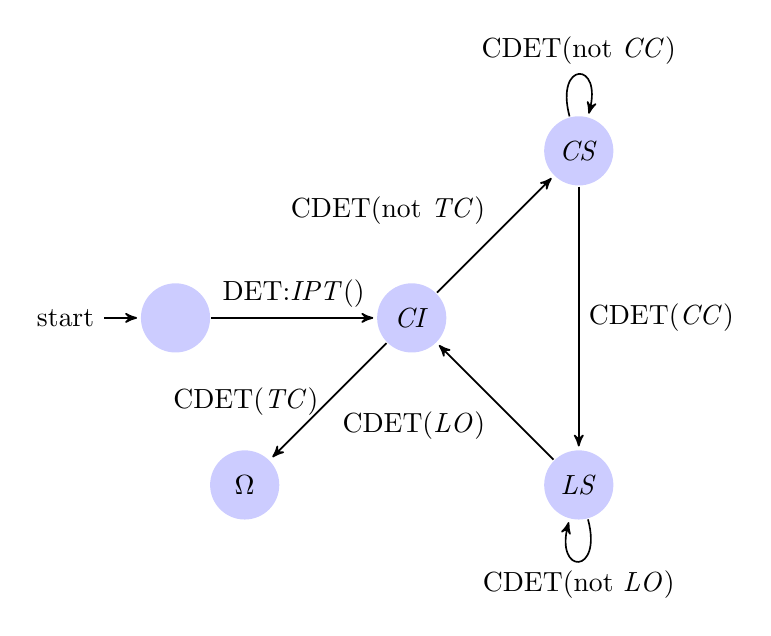
\begin{tikzpicture}[->,>=stealth',shorten >=1pt,auto,node distance=3cm,
                    semithick]
  \tikzstyle{every state}=[fill=blue!20,draw=none,thick]

  \node[initial,state]    (Init)                   {};
  \node[state]            (CI) [right of=Init]     {\emph{CI}};
  \node[state]            (CS) [above right of=CI] {\emph{CS}};
  \node[state]            (LS) [below right of=CI] {\emph{LS}};
  \node[state,accepting]  (End)[below left of=CI]  {$\Omega$};

  \path (Init) edge              node {DET:\emph{IPT}()} (CI)
        (CI) edge              node {CDET(not \emph{TC})} (CS)
             edge [left]       node {CDET(\emph{TC})} (End)
        (CS) edge [loop above] node {CDET(not \emph{CC})} (CS)
            edge              node {CDET(\emph{CC})} (LS)
        (LS) edge [loop below] node {CDET(not \emph{LO})} (LS)
            edge               node {CDET(\emph{LO})} (CI);
\end{tikzpicture}
\end{minipage}%
\hspace{1.5cm}
\begin{minipage}{.45\textwidth}
\centering
\paragraph{Nodes}
\begin{itemize}
  \item \emph{CI} $\equiv$ Dummy node
  \item \emph{CS} $\equiv$ \emph{ConstructSolution}($\alpha,\beta$)
  \item \emph{LS} $\equiv$ \emph{IterativeImprovementIBI}()
\end{itemize}
\paragraph{Conditions}
\begin{itemize}
  \item \emph{IPT} $\equiv$ \emph{InitializePheromoneTrail}()
  \item \emph{CC} $\equiv$ \emph{ConstructionComplete}()
  \item \emph{LO} $\equiv$ \emph{LocalOptimum}()
  \item \emph{TC} $\equiv$ \emph{TerminationCondition}($s,t_{max},f_{best}$)
\end{itemize}
\end{minipage}
\captionof{figure}{\maxmin  Ant System GLSM}
\end{center}

\newpage
In the implementation, an instance is completely defined by:
\begin{itemize}
\item \textbf{Cost matrix} - Encapsulating information on the node set $N$, edge set $E$, and weighting of each edge $c$.
\item \textbf{Time window vector} - Describing the time window mapping function $t$ for each node.
\end{itemize}

\subsubsection{Pheromone Initialization}
\begin{algorithm}[!h]
  \caption{Pheromone Initialization}\label{init}
  \begin{algorithmic}[1]
    \Procedure{InitalizePheromoneTrail}{$\tau_0,n_{cities}$}
      \State $\tau_{\max} \gets $
      \State $\tau_{\min} \gets $
      \State $i \gets 0$
      \State $j \gets 0$
      \For{$i < n_{cities}$} 
        \For{$j < i$} 
          \State $\tau_{ij} \gets \tau_0$
          \State $\tau_{ji} \gets \tau_{ij}$
          \State $ j \gets j + 1$  
        \EndFor
        \State $ i \gets i + 1$ 
      \EndFor
    \EndProcedure
\end{algorithmic}
\end{algorithm}

As discussed in \nameref{sec:introACO}, the ACO methods are based on stigmergic communication among the agents by means of virtual pheromone.

While the real ants can deposit pheromone anywhere in the environment, the virtual ants may only exchange information concerning solutions components.

For this reason, every admissible edge $e_{i,j}$ of $E$ has an associated pheromone value $\tau_{i,j}$, that have to be initialized at the beginning of the execution of the algorithm.

The initialization value $\tau_0$ is a parameter of the algorithm, for the \maxmin Ant System $\tau_0 = \tau_{i,j}(0) = \tau_{\max}$. 


\subsubsection{Solution construction}
\begin{algorithm}[!h]
  \caption{Solution Construction}\label{sol}
  \begin{algorithmic}[1]
    \Procedure{ConstructSolution}{$\alpha,\beta$}\Comment{The main procedure}
      \State \Comment{$s_i$ reprents the $i^{th}$ component of the solution}
      \State $s_0 \gets 0$ \Comment{Every solution starts at the depot}
      \State $s_1 \gets$ \emph{RandomCitySelection}() \Comment{Random choice of the starting city}
      \State $i \gets 1$
      \While{!\emph{SolutionComplete}()}
        \State $s_i \gets $ \emph{RouletteWheelSelection}() \Comment{ $s_i$ stochastically chosen according to the probability distribution defined by \ref{eq:tranprob}} 
        \State $i \gets i+1$
      \EndWhile
    \EndProcedure
\end{algorithmic}
\end{algorithm}

The solution construction process, used by every ant $k$ in the system, consist of a probabilistic selection of solution components.
Every edge $e_{i,j}$ has a selection probability $p_{i,j}^k(t)$ (also called transition probability) defined as follows:

\begin{equation} \label{eq:tranprob}
p_{i,j}^k(t) = \begin{cases}
  \frac{[\tau_{i,j}(t)]^\alpha \cdot [\eta_{i,j}]^\beta}{\sum_{k} \in A(s_{i}) [\tau_{k,j}(t)]^\alpha \cdot [\eta_{k,j}]^\beta} & j \in A(s_{i}) \\
 0 & \text{otherwise} \\
\end{cases}
\end{equation}

As one can see in \ref{eq:tranprob}, the transition probability is determined by a constant, locally available heuristic information $\eta_{i,j}$ and by the time varying pheromone trail $\tau_{i,j}(t)$.
This probability is defined on the set $A(s_i)$ of available (i.e. not yet visited) cities while visiting solution component $s_i$.
The value of the parameters $\alpha$ and $\beta$ determines the relative importance of the heuristic information and the pheromone trail, respectively.

\subsubsection{Solution improvement}
\begin{algorithm}[!h]
  \caption{Solution improvement}\label{sol}
  \begin{algorithmic}[1]
    \Procedure{IsImproving}{$s,s'$}\Comment{The main procedure}
      \If {$\Omega(s') < \Omega(s)$}
          \State \textbf{return true}
      \Else
           \If {$\Omega(s') = \Omega(s) \wedge f(s') < f(s)$}
            \State \textbf{return true}
           \EndIf
      \EndIf
      \State \textbf{return false}
      \EndProcedure
\end{algorithmic}
\end{algorithm}

A solution $s'$ is considered improving the current best solution $s$ if and only if:
\begin{itemize}
  \item Either,it has a smaller number of constraints violation (i.e. $\Omega(s') < \Omega(s)$)
  \item Or, it has the same number of constraints violations ($\Omega(s') == \Omega(s)$) but the total tour duration is smaller ($f(s') < f(s)$).
\end{itemize}


\subsubsection{Admissible heuristics}
The heuristic component $\eta_{i,j}$ is used to guide the selection of solution components towards those components that are included in optimal solution.

\paragraph{Dorigo et al, 1996}
The heuristic originally proposed by Dorigo et al, in \cite{dorigo1996ant}, for the TSP problem is:
\begin{equation}
  \eta_{i,j} = \frac{1}{c(e_{i,j})}
\end{equation}

The main idea behind this heuristic is that, if the selection process tends to select, at each step, the shortest connection between the current node and the following, the built tour should be of the shortest length.
This heuristic is cited for explanation purposes, even though it cannot be used for the TSPTW problem, since it will guide the exploration only towards shorter solutions, without taking into account the presence of the time windows.

\paragraph{Cheng and Mao, 2007}
The local heuristics used in \cite{cheng2007modified} are similar to that proposed by Gambardella et al. \cite{gambardella1999macs} in their multiple ant colony system (MACS) designed to solve the vehicle routing problem with time windows (VRPTW).

\begin{equation}
[\eta_{i,j}]^\beta = [g_{i,j}]^\beta \cdot [h_{i,j}]^\gamma
\end{equation}  

The two components $g_{i,j}$ and $h_{i,j}$, are designed, respectively, to avoid lateness (that is, arriving in the node where the time windows is already terminated) and waiting times (i.e. arriving in the node before the time windows open).

\subparagraph{Lateness avoidance}
\begin{equation}
g_{i,j} = \begin{cases}
 \frac{1}{1+e^{\delta \cdot (G_{i,j} - \mu)}}  &  G_{i,j} = b_j - t_j \geq 0 \\
0 & \text{otherwise} \\
\end{cases}
\end{equation}
where
\begin{itemize}
  \item $G_{i,j} = b_j - t_j$ - Slack corresponding to the time window $j$ while being in node $i$
  \item $t_i$ - Arrival time at node $i$
  \item $b_i$ - Closing time of time window $i$
  \item $G(i) = \{k\text{ } | \text{ }G_{i,k} \geq 0\}$ - Set of feasible neighbors of node $i$ (i.e. such that node $k$ is reached earlier than its closing time)
  \item $\mu = \frac{1}{|G(i)|}\sum_{j \in G(i)}  G_{i,j}$ - Average slack 
  \item $\delta$ - Parameter to control the slope of the sigmoidal function
\end{itemize}

\subparagraph{Waiting time avoidance}
\begin{equation}
h_{i,j} = \begin{cases}
 \frac{1}{1+e^{\lambda \cdot (H_{i,j} - \upsilon)}}  &  H_{i,j} = t_j - a_j \geq 0 \\
0 & \text{otherwise} \\
\end{cases}
\end{equation}
where
\begin{itemize}
  \item $H_{i,j} = t_j - a_j$ - Waiting time corresponding to the time window $j$ while being in node $i$
  \item $t_i$ - Arrival time at node $i$
  \item $a_i$ - Opening time of time window $i$
  \item $H(i) = \{k\text{ } | \text{ }H_{i,k} \geq 0\}$ - Set of non-waiting neighbors of node $i$ (i.e such that node $k$ is reached within the time window)
  \item $\upsilon = \frac{1}{|H(i)|}\sum_{j \in H(i)}  H_{i,j}$ - Average waiting time 
  $\lambda$ - Parameter to control the slope of the sigmoidal function 
\end{itemize}


\paragraph{Lopez-Ibanez and Blum, 2010}
The approach used in \cite{lopez2010beam} is a linear combination based on $\lambda_i$ coefficients, of the normalized values of opening and closing times of the time windows and the travelling cost from one city to another.

\begin{equation} \label{eq:heuristic}
\eta_{i-1,k} = \lambda_{a} \cdot \frac{a_{\max}-a_{k}}{a_{\max}-a_{\min}} + \lambda_{b} \cdot \frac{b_{\max}-b_{k}}{b_{\max}-b_{\min}} + \lambda_{c} \cdot \frac{c_{\max}-c_{i-1,k}}{c_{\max}-c_{\min}}
\end{equation}

where
\begin{itemize}
  \item $a_i$ - Opening time of time window $i$
  \item $a_{\max} = \max_{j \in N} a_{j}$ - Maximum time window opening time in the neighborhood of node $i$
  \item $a_{\min} = \min_{j \in N} a_{j}$ - Minimum time window opening time in the neighborhood of node $i$
  \item $b_i$ - Closing time of time window $i$
  \item $b_{\max} = \max_{j \in N} b_{j}$ - Maximum time window closing time in the neighborhood of node $i$
  \item $b_{\min} = \min_{j \in N} b_{j}$ - Minimum time window closing time in the neighborhood of node $i$
  \item $c_{i,j}$ - Travelling cost from node $i$ to node $j$
  \item $c_{\max} = \max_j c_{i,j}$ - Maximum travelling cost from node $i$ 
  \item $c_{\min} = \min_j c_{i,j}$ - Minimum travelling cost from node $i$
  \item $\lambda_{a},\lambda_{b},\lambda_{c}$ s.t. $\lambda_{a}+\lambda_{b}+\lambda_{c}=1$ - Randomly selected weights
\end{itemize}

In this implementation, the heuristic information will be computed according to \cite{lopez2010beam}

\subsubsection{Pheromone trails update}
\begin{algorithm}[!h]
  \caption{Pheromone Trails Update}\label{update}
  \begin{algorithmic}[1]
    \Procedure{UpdatePheromoneTrails}{$\rho,p_b$}\Comment{The main procedure}
     \State $i \gets 0$
      \State $j \gets 0$
      \For{$i < n_{cities}$} 
        \For{$j < i$}
          \If{\emph{Random}() $< \varepsilon$} 
          \State $\tau_{ij} \gets (1-\rho)\cdot\tau_{ij}+\Delta\tau_{i,j}^{Bi}$
          \Else
          \State $\tau_{ij} \gets (1-\rho)\cdot\tau_{ij}+\Delta\tau_{i,j}^{Bo}$
          \EndIf
          \If{$\tau_{ij} < \tau_{\min}$} 
            \State $\tau_{ij} \gets \tau_{\min}$
          \EndIf
          \If{$\tau_{ij} > \tau_{\max}$} 
            \State $\tau_{ij} \gets \tau_{\max}$
          \EndIf
          \State $\tau_{ji} \gets \tau_{ij}$
          \State $ j \gets j + 1$  
        \EndFor
        \State $ i \gets i + 1$ 
      \EndFor
    \EndProcedure
\end{algorithmic}
\end{algorithm}

As discussed in \nameref{sec:algstrucACO}, the pheromone update will be made by a single ant, being either the one who found the best solution in the current iteration: 

\begin{equation}
  \Delta\tau_{i,j}^{Bi} = \begin{cases}
    \frac{1}{T_{d}^{\text{Bi}}} & e_{i,j} \in T^{\text{Bi}}  \\
    0 & \text{otherwise} 
      \end{cases}
\end{equation}

Or the one having found the global best (best-so-far) solution:

\begin{equation}
  \Delta\tau_{i,j}^{Bo} = \begin{cases}
    \frac{1}{T_{d}^{\text{Bo}}} & e_{i,j} \in T^{\text{Bo}}  \\
    0 & \text{otherwise} 
  \end{cases}
\end{equation}

where
\begin{itemize}
\item $e_{i,j}$ - Edge connecting node $i$ and $j$
\item $T_{d}^{i}$ - Complete tour duration of tour $i$
\item $T^{\text{Bi}}$ - Best tour of the current iteration
\item $T^{\text{Bo}}$ - Best tour overall 
\end{itemize}


Provided that the best solution is known, the bounds on the pheromone values can be estimated by:
\begin{equation}
\begin{array}{lccr}
  \hat{\tau}_{\max} = \frac{1}{\rho \cdot T_{d}^{\text{Go}}} & & & \hat{\tau}_{\min} = \frac{\hat{\tau}_{\max}}{a}
\end{array}
\end{equation}

\subsubsection{Local search}
\begin{algorithm}[!h]
  \caption{Iterative Improvement - (Insert neighborhood with best improve pivoting rule)}\label{locsearch}
  \begin{algorithmic}[1]
    \Procedure{IterativeImprovementIBI}{$s$}\Comment{The main procedure}
      \State $s^{*} \gets s$ 
      \For {$i \in \{1,\cdots,|N|\}$}
        \For {$j \in \{1,\cdots,|N|\}$}
          \If{ $i = j \vee  j = i-1 $}
				    \State \textbf{continue}
			    \EndIf
			    \State $s' \gets$ \emph{InsertTourComponent}($s,i,j$)
			    \If {\emph{IsImproving}($s^{*},s'$)}
          \State $s^{*} \gets s'$
        \EndIf
        \EndFor
      \EndFor
      \State \textbf{return} $s^{*}$
    \EndProcedure
\end{algorithmic}
\end{algorithm}

\begin{algorithm}[!h]
  \caption{Insert neighbor solution computation}\label{locsearch}
  \begin{algorithmic}[1]
    \Procedure{InsertTourComponent}{$s,i,j$}\Comment{The main procedure}
      \State \Comment{$s_i$ reprents the $i^{th}$ component of the solution}
      \State $e \gets s_i$
      \If{i<j}
      \State $k \gets i$
        \While{$k < j$}
				  \State $s_i \gets s_{i+1}$
				  \State $k \gets k+1$
			  \EndWhile
			\Else
			\State $k \gets i$
        \While{$k > j$}
				  \State $s_i \gets s_{i-1}$
				  \State $k \gets k-1$
			  \EndWhile
			\EndIf
			\State $s_j \gets e$
     \State \textbf{return} $s$
    \EndProcedure
\end{algorithmic}
\end{algorithm}


The solution construction process, used by every ant $k$ in the system, consist of a probabilistic selection of solution components.
Every edge $e_{i,j}$ has a selection probability $p_{i,j}^k(t)$ (also called transition probability) defined as follows:

\begin{equation} 
p_{i,j}^k(t) = \begin{cases}
  \frac{[\tau_{i,j}(t)]^\alpha \cdot [\eta_{i,j}]^\beta}{\sum_{k} \in A(s_{i}) [\tau_{k,j}(t)]^\alpha \cdot [\eta_{k,j}]^\beta} & j \in A(s_{i}) \\
 0 & \text{otherwise} \\
\end{cases}
\end{equation}

As one can see in \ref{eq:tranprob}, the transition probability is determined by a constant, locally available heuristic information $\eta_{i,j}$ and by the time varying pheromone trail $\tau_{i,j}(t)$.
This probability is defined on the set $A(s_i)$ of available (i.e. not yet visited) cities while visiting solution component $s_i$.
The value of the parameters $\alpha$ and $\beta$ determines the relative importance of the heuristic information and the pheromone trail, respectively.

\subsubsection{Termination condition}
\begin{algorithm}[!h]
  \caption{Termination Condition}\label{termcond}
  \begin{algorithmic}[1]
    \Procedure{TerminationCondintion}{$s,t_{\max},s_{best}$}
          \If{ $(f(s) = f_{best} \wedge \Omega(s) = 0) \vee  t > t_{\max} $}
				    \State \textbf{return true}
			    \EndIf
      \State \textbf{return false}
    \EndProcedure
\end{algorithmic}
\end{algorithm}

\subsubsection{Implementation parameters}
\begin{center}
\begin{tabular}{|c|c|c|}
\hline
\textbf{Parameter} & \textbf{Default} & \textbf{Selected} \\ \hline 
$\alpha$ & 1.0 & 1.0 \\\hline
$\beta$ & 2.0 & 2.0 \\\hline 
$\tau_0$ & 1.0 & 1.0 \\ \hline
$\varepsilon$ & 0.5 & 0.5 \\ \hline 
$Ants$ & 25 & 25 \\ \hline  
$t_{\max}$ & 10[s] & 10[s] \\ \hline
\end{tabular}
\captionof{table}{SA - Algorithm parameters overview}
\label{saParameters}
\end{center}

 
\end{homeworkProblem}

%%----------------------------------------------------------------------------------------
%	PROBLEM 1
%----------------------------------------------------------------------------------------

% To have just one problem per page, simply put a \clearpage after each problem
\newpage
\begin{homeworkProblem}
\section{Variable neighborhood descent algorithms}
\subsection{Problem statement}
Implement both a standard and piped variable neighborhood descent (VND) algorithm (concatenation of the underlying iterative improvement algorithms; see lecture slides). Consider the two possible (reasonable) orderings of
the iterative improvement algorithms (indicated by the neighborhood relation they use):
\begin{itemize}
  \item transpose, exchange, insert
  \item transpose, insert, exchange 
\end{itemize}
Implement the 4 VND algorithms (all combinations of standard and piped and the two neighborhood orders) using first-improvement and random initialization.

\subsection{Experiment results}
\subsubsection{n80w20.001}
\begin{center}
\includegraphics[width=0.6\textwidth,keepaspectratio]{{VND/n80w20.001/n80w20.001-CpuTime}.pdf}
\captionof{figure}{n80w20.001 - Runtime boxplots for the different variable neighborhood descent algorithms}
\end{center}

\begin{center}
\includegraphics[width=0.6\textwidth,keepaspectratio]{{VND/n80w20.001/n80w20.001-PRPD}.pdf}
\captionof{figure}{n80w20.001 - PRPD boxplots for the different variable neighborhood descent algorithms}
\end{center}

\begin{center}
\begin{tabular}{|l|l|}
\hline
\textbf{Test} & \textbf{P-Value} \\
\hline
Tei vs Tie - Standard&3.95591160889952e-18\\
\hline
Tei vs Tie - Piped&3.9556885406462e-18\\
\hline
Standard vs Piped - Tei&3.95591160889952e-18\\
\hline
Standard vs Piped - Tie&3.95591160889952e-18\\
\hline
\end{tabular}
\captionof{table}{n80w20.001 - Results of Wilcoxon paired signed rank test}
\end{center}

\subsubsection{n80w20.002}
\begin{center}
\includegraphics[width=0.6\textwidth,keepaspectratio]{{VND/n80w20.002/n80w20.002-CpuTime}.pdf}
\captionof{figure}{n80w20.002 - Runtime boxplots for the different variable neighborhood descent algorithms}
\end{center}

\begin{center}
\includegraphics[width=0.6\textwidth,keepaspectratio]{{VND/n80w20.002/n80w20.002-PRPD}.pdf}
\captionof{figure}{n80w20.002 - PRPD boxplots for the different variable neighborhood descent algorithms}
\end{center}

\begin{center}
\begin{tabular}{|l|l|}
\hline
\textbf{Test} & \textbf{P-Value} \\
\hline
Tei vs Tie - Standard&3.9556885406462e-18\\
\hline
Tei vs Tie - Piped&3.95591160889952e-18\\
\hline
Standard vs Piped - Tei&3.95591160889952e-18\\
\hline
Standard vs Piped - Tie&3.95591160889952e-18\\
\hline
\end{tabular}
\captionof{table}{n80w20.002 - Results of Wilcoxon paired signed rank test}
\end{center}

\subsubsection{n80w20.003}
\begin{center}
\includegraphics[width=0.6\textwidth,keepaspectratio]{{VND/n80w20.003/n80w20.003-CpuTime}.pdf}
\captionof{figure}{n80w20.003 - Runtime boxplots for the different variable neighborhood descent algorithms}
\end{center}

\begin{center}
\includegraphics[width=0.6\textwidth,keepaspectratio]{{VND/n80w20.003/n80w20.003-PRPD}.pdf}
\captionof{figure}{n80w20.003 - PRPD boxplots for the different variable neighborhood descent algorithms}
\end{center}

\begin{center}
\begin{tabular}{|l|l|}
\hline
\textbf{Test} & \textbf{P-Value} \\
\hline
Tei vs Tie - Standard&3.9552424399092e-18\\
\hline
Tei vs Tie - Piped&3.95591160889952e-18\\
\hline
Standard vs Piped - Tei&3.95591160889952e-18\\
\hline
Standard vs Piped - Tie&3.95591160889952e-18\\
\hline
\end{tabular}
\captionof{table}{n80w20.003 - Results of Wilcoxon paired signed rank test}
\end{center}

\subsubsection{n80w20.004}
\begin{center}
\includegraphics[width=0.6\textwidth,keepaspectratio]{{VND/n80w20.004/n80w20.004-CpuTime}.pdf}
\captionof{figure}{n80w20.004 - Runtime boxplots for the different variable neighborhood descent algorithms}
\end{center}

\begin{center}
\includegraphics[width=0.6\textwidth,keepaspectratio]{{VND/n80w20.004/n80w20.004-PRPD}.pdf}
\captionof{figure}{n80w20.004 - PRPD boxplots for the different variable neighborhood descent algorithms}
\end{center}

\begin{center}
\begin{tabular}{|l|l|}
\hline
\textbf{Test} & \textbf{P-Value} \\
\hline
Tei vs Tie - Standard&3.95591160889952e-18\\
\hline
Tei vs Tie - Piped&3.95591160889952e-18\\
\hline
Standard vs Piped - Tei&3.95591160889952e-18\\
\hline
Standard vs Piped - Tie&3.95591160889952e-18\\
\hline
\end{tabular}
\captionof{table}{n80w20.004 - Results of Wilcoxon paired signed rank test}
\end{center}

\subsubsection{n80w20.005}
\begin{center}
\includegraphics[width=0.6\textwidth,keepaspectratio]{{VND/n80w20.005/n80w20.005-CpuTime}.pdf}
\captionof{figure}{n80w20.005 - Runtime boxplots for the different variable neighborhood descent algorithms}
\end{center}

\begin{center}
\includegraphics[width=0.6\textwidth,keepaspectratio]{{VND/n80w20.005/n80w20.005-PRPD}.pdf}
\captionof{figure}{n80w20.001 - PRPD boxplots for the different variable neighborhood descent algorithms}
\end{center}

\begin{center}
\begin{tabular}{|l|l|}
\hline
\textbf{Test} & \textbf{P-Value} \\
\hline
Tei vs Tie - Standard&3.95591160889952e-18\\
\hline
Tei vs Tie - Piped&3.95591160889952e-18\\
\hline
Standard vs Piped - Tei&3.95591160889952e-18\\
\hline
Standard vs Piped - Tie&3.95591160889952e-18\\
\hline
\end{tabular}
\captionof{table}{n80w20.005 - Results of Wilcoxon paired signed rank test}
\end{center}

\subsubsection{n80w200.001}
\begin{center}
\includegraphics[width=0.6\textwidth,keepaspectratio]{{VND/n80w200.001/n80w200.001-CpuTime}.pdf}
\captionof{figure}{n80w200.001 - Runtime boxplots for the different variable neighborhood descent algorithms}
\end{center}

\begin{center}
\includegraphics[width=0.6\textwidth,keepaspectratio]{{VND/n80w200.001/n80w200.001-PRPD}.pdf}
\captionof{figure}{n80w200.001 - PRPD boxplots for the different variable neighborhood descent algorithms}
\end{center}

\begin{center}
\begin{tabular}{|l|l|}
\hline
\textbf{Test} & \textbf{P-Value} \\
\hline
Tei vs Tie - Standard&4.07730530936212e-18\\
\hline
Tei vs Tie - Piped&2.92094064174088e-17\\
\hline
Standard vs Piped - Tei&2.72456795287507e-16\\
\hline
Standard vs Piped - Tie&3.95591160889952e-18\\
\hline
\end{tabular}
\captionof{table}{n80w200.001 - Results of Wilcoxon paired signed rank test}
\end{center}

\subsubsection{n80w200.002}
\begin{center}
\includegraphics[width=0.6\textwidth,keepaspectratio]{{VND/n80w200.002/n80w200.002-CpuTime}.pdf}
\captionof{figure}{n80w200.002 - Runtime boxplots for the different variable neighborhood descent algorithms}
\end{center}

\begin{center}
\includegraphics[width=0.6\textwidth,keepaspectratio]{{VND/n80w200.002/n80w200.002-PRPD}.pdf}
\captionof{figure}{n80w200.002 - PRPD boxplots for the different variable neighborhood descent algorithms}
\end{center}

\begin{center}
\begin{tabular}{|l|l|}
\hline
\textbf{Test} & \textbf{P-Value} \\
\hline
Tei vs Tie - Standard&3.95591160889952e-18\\
\hline
Tei vs Tie - Piped&1.52379449675399e-17\\
\hline
Standard vs Piped - Tei&1.74838327736385e-15\\
\hline
Standard vs Piped - Tie&3.95591160889952e-18\\
\hline
\end{tabular}
\captionof{table}{n80w200.002 - Results of Wilcoxon paired signed rank test}
\end{center}

\subsubsection{n80w200.003}
\begin{center}
\includegraphics[width=0.6\textwidth,keepaspectratio]{{VND/n80w200.003/n80w200.003-CpuTime}.pdf}
\captionof{figure}{n80w200.003 - Runtime boxplots for the different variable neighborhood descent algorithms}
\end{center}

\begin{center}
\includegraphics[width=0.6\textwidth,keepaspectratio]{{VND/n80w200.003/n80w200.003-PRPD}.pdf}
\captionof{figure}{n80w200.003 - PRPD boxplots for the different variable neighborhood descent algorithms}
\end{center}

\begin{center}
\begin{tabular}{|l|l|}
\hline
\textbf{Test} & \textbf{P-Value} \\
\hline
Tei vs Tie - Standard&2.04955667109233e-17\\
\hline
Tei vs Tie - Piped&2.59611565456869e-17\\
\hline
Standard vs Piped - Tei&1.50422804122146e-07\\
\hline
Standard vs Piped - Tie&3.95591160889952e-18\\
\hline
\end{tabular}
\captionof{table}{n80w200.003 - Results of Wilcoxon paired signed rank test}
\end{center}

\subsubsection{n80w200.004}
\begin{center}
\includegraphics[width=0.6\textwidth,keepaspectratio]{{VND/n80w200.004/n80w200.004-CpuTime}.pdf}
\captionof{figure}{n80w200.004 - Runtime boxplots for the different variable neighborhood descent algorithms}
\end{center}

\begin{center}
\includegraphics[width=0.6\textwidth,keepaspectratio]{{VND/n80w200.004/n80w200.004-PRPD}.pdf}
\captionof{figure}{n80w200.004 - PRPD boxplots for the different variable neighborhood descent algorithms}
\end{center}

\begin{center}
\begin{tabular}{|l|l|}
\hline
\textbf{Test} & \textbf{P-Value} \\
\hline
Tei vs Tie - Standard&4.07730530936212e-18\\
\hline
Tei vs Tie - Piped&4.29577057320019e-16\\
\hline
Standard vs Piped - Tei&5.3075517052254e-11\\
\hline
Standard vs Piped - Tie&3.95591160889952e-18\\
\hline
\end{tabular}
\captionof{table}{n80w200.004 - Results of Wilcoxon paired signed rank test}
\end{center}

\subsubsection{n80w200.005}
\begin{center}
\includegraphics[width=0.6\textwidth,keepaspectratio]{{VND/n80w200.005/n80w200.005-CpuTime}.pdf}
\captionof{figure}{n80w200.005 - Runtime boxplots for the different variable neighborhood descent algorithms}
\end{center}

\begin{center}
\includegraphics[width=0.6\textwidth,keepaspectratio]{{VND/n80w200.005/n80w200.005-PRPD}.pdf}
\captionof{figure}{n80w200.001 - PRPD boxplots for the different variable neighborhood descent algorithms}
\end{center}

\begin{center}
\begin{tabular}{|l|l|}
\hline
\textbf{Test} & \textbf{P-Value} \\
\hline
Tei vs Tie - Standard&1.39380002081336e-17\\
\hline
Tei vs Tie - Piped&4.07730530936212e-18\\
\hline
Standard vs Piped - Tei&3.72316935219101e-06\\
\hline
Standard vs Piped - Tie&3.95591160889952e-18\\
\hline
\end{tabular}
\captionof{table}{n80w200.001 - Results of Wilcoxon paired signed rank test}
\end{center}

\subsection{Statistics}
\subsubsection{Standard-Transpose-Exchange-Insert}
\begin{center}
\begin{tabular}{|l|c|l|l|}
\hline
\textbf{Instance}& \textbf{\% Infeasible} & $\mathbf{\bar{PRDP}}$ &$\mathbf{\bar{Runtime}}$\\
\hline
n80w20.001&0.71&14772.04644164&50.611339\\
\hline
n80w20.002&0.88&12888.542&50.727053\\
\hline
n80w20.003&0.92&19936.872&50.820348\\
\hline
n80w20.004&0.62&17234.94260984&50.049484\\
\hline
n80w20.005&0.94&12564.0560428&50.269182\\
\hline
n80w200.001&0.28&11212.97389136&49.151249\\
\hline
n80w200.002&0.03&629.5853274&51.433949\\
\hline
n80w200.003&0.07&1511.56628539&49.082085\\
\hline
n80w200.004&0.16&4193.4817209&49.662512\\
\hline
n80w200.005&0.01&466.6729061&46.701953\\
\hline

\end{tabular}
\captionof{table}{Statistics summary for variable neighborhood descent algorithm with Transpose-Exchange-Insert neighborhood chain and Standard VND type}
\end{center}

\subsubsection{Standard-Transpose-Insert-Exchange}
\begin{center}
\begin{tabular}{|l|c|l|l|}
\hline
\textbf{Instance}& \textbf{\% Infeasible} & $\mathbf{\bar{PRDP}}$ &$\mathbf{\bar{Runtime}}$\\
\hline
n80w20.001&0.54&10874.77632472&15.268454\\
\hline
n80w20.002&0.62&8411.724&15.386641\\
\hline
n80w20.003&0.44&7645.295&15.638153\\
\hline
n80w20.004&0.39&7153.68881324&15.980347\\
\hline
n80w20.005&0.25&3475.2731712&15.55767\\
\hline
n80w200.001&0.16&4898.3227617&33.424555\\
\hline
n80w200.002&0&11.0430351&32.198479\\
\hline
n80w200.003&0.05&1082.1460308&34.345522\\
\hline
n80w200.004&0.28&7804.19186258&32.583152\\
\hline
n80w200.005&0&10.20227353&34.501294\\
\hline


\end{tabular}
\captionof{table}{Statistics summary for variable neighborhood descent algorithm with Transpose-Insert-Exchange neighborhood chain and Standard VND type}
\end{center}

\subsubsection{Piped-Transpose-Exchange-Insert}
\begin{center}
\begin{tabular}{|l|c|l|l|}
\hline
\textbf{Instance}& \textbf{\% Infeasible} & $\mathbf{\bar{PRDP}}$ &$\mathbf{\bar{Runtime}}$\\
\hline
n80w20.001&0.59&12336.84228578&35.694416\\
\hline
n80w20.002&0.94&15603.0142035&36.212393\\
\hline
n80w20.003&0.83&19338.924&34.821217\\
\hline
n80w20.004&0.55&13170.33921962&36.438959\\
\hline
n80w20.005&0.45&6683.336214&36.202891\\
\hline
n80w200.001&0.19&5104.3621015&40.772642\\
\hline
n80w200.002&0.01&218.8179842&44.241593\\
\hline
n80w200.003&0.06&2584.90674231&44.725066\\
\hline
n80w200.004&0.17&3430.64506042&43.760992\\
\hline
n80w200.005&0.02&693.0136326&42.646023\\
\hline

\end{tabular}
\captionof{table}{Statistics summary for variable neighborhood descent algorithm with Transpose-Exchange-Insert neighborhood chain and Standard VND type}
\end{center}

\subsubsection{Piped-Transpose-Insert-Exchange}
\begin{center}
\begin{tabular}{|l|c|l|l|}
\hline
\textbf{Instance}& \textbf{\% Infeasible} & $\mathbf{\bar{PRDP}}$ &$\mathbf{\bar{Runtime}}$\\
\hline
n80w20.001&0.68&16393.81210394&24.788225\\
\hline
n80w20.002&0.81&11667.654&25.902581\\
\hline
n80w20.003&0.84&20537.669&26.442309\\
\hline
n80w20.004&0.46&8779.79314651&26.424231\\
\hline
n80w20.005&0.24&3876.3661498&26.511156\\
\hline
n80w200.001&0.21&5917.0312803&52.302366\\
\hline
n80w200.002&0.01&626.0983757&56.238843\\
\hline
n80w200.003&0.04&867.92563269&58.498874\\
\hline
n80w200.004&0.28&6281.58944822&55.867038\\
\hline
n80w200.005&0.01&236.8657243&58.331595\\
\hline

\end{tabular}
\captionof{table}{Statistics summary for variable neighborhood descent algorithm with Transpose-Insert-Exchange neighborhood chain and Standard VND type}
\end{center}

\end{homeworkProblem}



\section{Conclusions}
By combining the results from the previous analysis:
\begin{itemize}
  \item The Iterative Improvement algorithms based on Transpose and Exchange neighborhoods do not allow to find feasible solutions hence they should not be considered for a practical application.
  \item On the other hand, the solution quality generated by the Iterative Improvement algorithm with the Insert neighborhood is similar to those generated by the VND algorithms, regardless of the instances.
  \item On this set of instances, the VND algorithms have a lower runtime than the Iterative Improvement one using Insert neighborhood, hence being similar the resulting solution quality, they should be preferred to the Iterative Improvement ones.
  \item The algorithm that showed the best performances in terms of solution quality and runtime is the Standard Variable Neighborhood Descent with Transpose-Insert-Exchange neighborhood chain.
  \item The usage of average statistics as metrics to measure the quality of the algorithms is strongly biased by the presence of outliers (penalisation, in this case).
\end{itemize}



\bibliographystyle{plain}
\bibliography{References}

\end{document}
